%!TEX root = ../dissertation.tex

\chapter{State Of The Art}
\label{chapter:state_art}

The growing demand for faster General-Purpose Processors (GPPs)  The improvement of computer speed and capabilities is a very broad area of investigation, with research focused on several areas, from faster computational units, like accelerators, to improvements in data access through pre-fetching, memory caching, and data streaming.



% Data Level paralelism


\section{Unlimited Vector Extention}

Unlimited Vector Extention is a novelty solution that aims to surpass the existing problems of current state-of-the-art solutions of scalable vector extensions, through the use of a data streaming engine, combining streaming and SIMD processing, which allows the exploitation of data parallelism.


The proposed ISA tries to reduce latencies associated with loop control, memory access indexing, and memory access through the use of new instructions that allow a pre-configuration of the stream and the memory access patterns. 
This anticipation of the access control allows for accurate and fast pre-fetching even with multidimensional arrays or indirect memory accesses. 


\subsection{Differentiation}
%The utilization of Single Instruction Multiple Data is not something new, however currently developed approaches focus on operation on fixed-size registers (e.g., Intel MMX, SSE, AVX, etc) this leads to an easier implementation and simplifies hardware requirements. 

%Other solutions have emerged allowing for a more agnostic approach to the physical vector size of registers from the point of view of the programmer. This implementation allows that, only at run time, the compiled software adapts to the given vector size of the system. ARM SVE and RISC-V Vector extension (RVV) are two of these types of implementations.

%The use of any of these solutions incurs the need to modify the active lanes of the vector achieving that through vector control instructions. The addition of these instructions to the iterations leads to an increase in the number of instructions which leads to higher latencies. 

\begin{figure}[H]
    \centering
    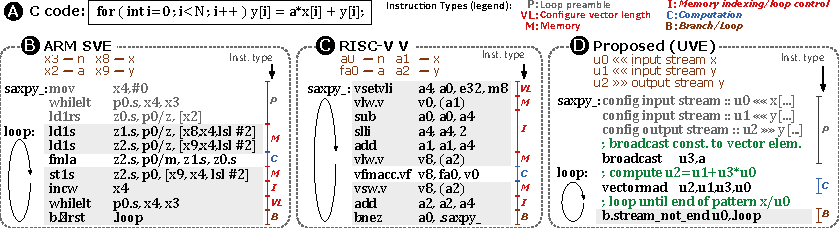
\includegraphics[width=0.77\linewidth]{images/UVE-Comparison.pdf}
    \caption{A boat.}
    \label{fig:uve-comparison}
\end{figure}

The distinguishability of this solution, from  currently developed SIMD solutions (ARM SVE and RISC-V Vector extension (RVV)) comes from features like:
\begin{itemize}
\item[]  \Tbullet{F1}{Decoupled Memory Access} The ability to decouple the memory accesses from the computation part by streaming the data directly to the register allowing the occurrence of loads/stores in parallel with the data manipulation thus reducing the memory access latency.
\item[]  \Tbullet{F2}{Indexing-free Loops} Describing the load/store patterns in advance, minimizing the number of instructions related to memory indexing, reducing the pressure on the processor pipeline (see the UVE Fig.\ref{fig:uve-comparison}.D. It also helps avoid the transfer of miss-predicted data.
\item[]  \Tbullet{F3}{Simpified Vectorization} The description of memory pattern access allows the Streaming Engine to perform all non-coalesced accesses as linear patterns. This leads to a simplified vectorization since memory is always aligned from the execution pipeline point of view - see Fig. \ref{fig:uve-mem-access}. 
\item[]  \Tbullet{F4}{Implicit Load/Store} Due to the description of the streams in the loop preamble, the indexing instructions can be removed meaning that all explicit loads and stores are simply associated with active streams and different vector register.
\end{itemize}

Besides the mentioned features, UVE is also register-size agnostic similar to SVE and RVV, however in UVE there is no need for control instruction since the Streaming Engine automatically disables all vector elements that fall out of bounds, making the loops simpler with a minimal set of control functions.


\begin{figure}[H]
	\begin{center}
 		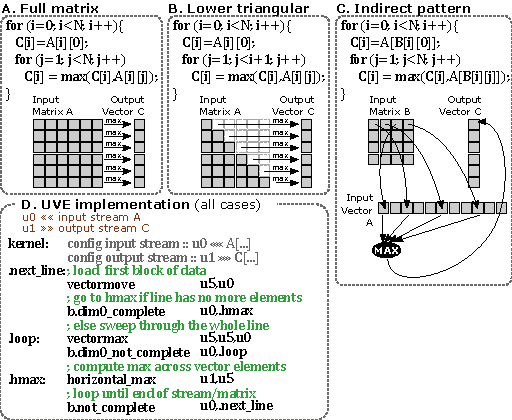
\includegraphics[width=0.37\linewidth]{images/memory-access.pdf}
 		\caption{Execution time for each configuration}
 		\label{fig:uve-mem-access}
	\end{center} 
\end{figure}

\subsection{Data Streaming}

The proposed UVE 



\section{ARM Scalable Vector Extention}
\section{Data-Prefetching}
\section{Stream Specialized Processor}
\section{Stream Semantic Registers}

% Data Streaming
% Memory Vectorization